\documentclass{article}
\usepackage[italian]{babel}
\usepackage{t1enc}
\usepackage{amsmath,amssymb}
\usepackage{amsthm}
\usepackage{graphicx}
\usepackage{a4wide}
\newtheorem{remark}{Remark}
\newtheorem{lineeguida}{Linee guida}
\author{Luca Formaggia}
\date{{PACS 20014-2015}\\
}
\title{A first example of c++ program}
\begin{document}
\section{Heat exchange in a one-dimensional bar}


We consider a bar of length $L$ and constant thermal conductivity $k$ (see figure).
One end of the bar is kept at constant temperature $T_0$, while the other end is under
adiabatic conditions (zero thermal flux).
The bar exchanges heat with the surrounding air at temperature $T_a$.  
Using a onedimensional model, the steady state solution 
satiefies
\begin{equation}
\label{eq:sto}
-k \frac{d^2}{dx^2}T + h_p(T-T_a)=0\quad 0<x<L,
\end{equation}
con condizioni al bordo date da
\begin{equation}
\label{eq:stobc}
T(0)=T_0\qquad \frac{d}{dx}T(L)=0.
\end{equation}

\begin{figure}
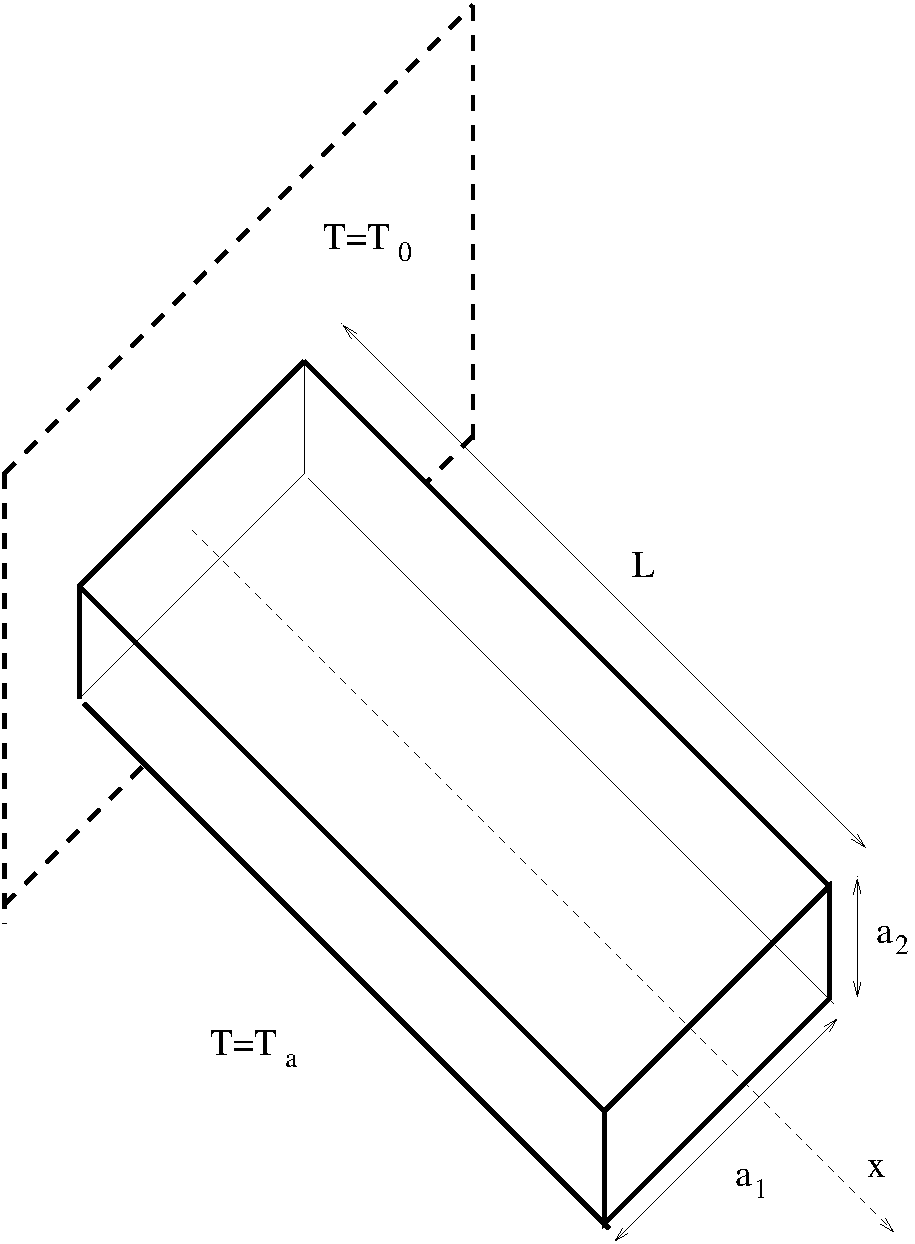
\includegraphics[width=0.6\textwidth]{Figure/barra}
\caption{The bar we are considering in this example. It exchanges heat
through one end, kept at constant temperature, and with the surrounding medium. The other end
is insulated.}
\end{figure}

The coefficient of convective heat exchange per unit length $h_p$
[W/m$^2$K] is assumed constant. It is linked to the coefficient per unit area 
$h$ [W/mK] by the relation
\[
h_p=\frac{hp}{S},
\]
$p$ being the perimeter and  $S$ the section of the bar. Since the bar has a rectangular section, 
with sides of length $a_1$ and $a_2$ we can write
\[
h_p=\frac{2h(a_1+a_2)}{a_1a_2}.
\]

Equations (\ref{eq:sto}) and (\ref{eq:stobc}) may be rewritten in terms of the 
temperature difference  $\theta=T-T_a$ and normalized by setting
\[
x \rightarrow x/L.
\]
Thus, in the following $x$ indicates the normalized (a-dimensional) abscissa and the domain becomes
the interval $(0,1)$. In the normalized variables the problem is
\begin{equation}
\label{eq:st}
-\frac{d^2}{dx^2}\theta +a\theta =0\quad 0<x<1,
\end{equation}
with boundary conditions
\begin{equation}
\label{eq:stbc}
\theta(0)=\theta_0=T_0-T_a\qquad \frac{d}{dx}\theta(1)=0,
\end{equation}
where
\[
a=\frac{L^2h_p}{k}=\frac{2L^2 h(a_1+a_2)}{ka_1a_2}.
\]

We consider a uniform grid of  $M$ elements in the interval 
$[0,1]$ and we discretize  (\ref{eq:st}) with linear finite elements.
We indicate with  $u_i=u_h(x_i)$, $i=0,\ldots,M$ the approximation of
$\theta$ at the nodes $x_i=h i$, being $h=1/M$.

The problem unknowns are given by $u_i$, $i=1,\ldots,M$, since, thanks to the boundary condition, 
$u_0=\theta_0$.  We operate  in the usual way to obtain a linear system
\begin{equation}
\label{eq:stfem}
A\mathbf{u}=\mathbf{b},
\end{equation}
with 
\[
\mathbf{u}=[u_1,\ldots,u_n]^T,\quad \mathbf{b}=[\theta_0,0,\ldots,0]^T
\]
and $A\in \mathbb{R}^{M\times M}$ the matrix given by
\[
A=\left[
\begin{array}{llllll}
2+h^2a & -1 & 0 &\ldots&\ldots& 0\\
-1 & 2+h^2a & -1 &\ldots&\ldots& 0\\
 &   & \ldots &\ldots& & \\
0  & \ldots & \ldots &-1 &2+h^2a& -1\\
0  & \ldots & \ldots &\ldots&-1& 1\\
\end{array}
\right].
\]

Matrix $A$ is symmetric positive definite, thus we may use the 
Gauss-Siedel iterative scheme for the solution of the linear system.

One may verify that the single iteration of Gauss-Siedel can be written as 
\[
u_i^{(k+1)}=\frac{u^{(k)}_{i-1}+u^{(k)}_{i+1}}{2+h^2a},\quad i=1,\ldots,M-1
\]
and
\[
u_M^{(k+1)}=u^{(k)}_{M-1},
\]
being $k$ the iteration index. We terminate the iterations when 
$||\mathbf{u}^{(k+1)}-\mathbf{u}^{(k)}||\le \tau$, for a given tolerance
$\tau>0$, or when  $k\ge k_{max}$ (no convergence within a maximal number of iterations $ k_{max}$).

\subsection{The exact solution}
The exact solution of problem (\ref{eq:st})-(\ref{eq:stbc})
is
\[
\theta(x)=\theta_0\frac{\cosh[\sqrt{a}(1-x)]}{\cosh(\sqrt{a})}.
\]

\subsection{The program heat\_exchange.cpp}
In the directory \texttt{Heat\_Exchange} you have a prototype program 
simply called 
\texttt{main.cpp} that solves the problem with the proposed numerical scheme. 

Is a simple program and it does use little use of advanced C++ programming.
It is not general, and difficult to extend to other finite elements or other numerical schemes for the solution of the linear system.

It is just a first example on which the students may elaborate further.
You have a \texttt{Makefile} that allow to compile the code by simply 
typing 
\texttt{make main} or just \texttt{make} in the  directory where the program is kept.

You may generate the executable directly, for instance with
\begin{verbatim}
g++ -std=c++11 -o main *.cpp
\end{verbatim}

The file \texttt{parameters.hpp} defines a struct with the default values
of the parameters, namely
\begin{tabular}{ccc|ccc}
\multicolumn{1}{c}{Variabile}&
\multicolumn{1}{c}{Nome nel pr.}&
\multicolumn{1}{c}{Valore}&
\multicolumn{1}{c}{Variabile}&
\multicolumn{1}{c}{Nome nel pr.}&
\multicolumn{1}{c}{Valore}
\\\hline
$L$ &\texttt{L}& $40$ &
$a_1$&\texttt{a1}&$4$\\
$a_2$ &\texttt{a2}& $50$ &
$T_0$&\texttt{To}&$46$\\
$T_a$ &\texttt{Te}& $20$ &
$k$&\texttt{k}&$0.164$\\
$h$ &\texttt{hc}& $200\times 10^{-6}$ &&&\\\hline
\end{tabular}.
Those values may be changed by using a \texttt{GetPot} file, the default
name being \texttt{Parameters.pot}.

The program accepts arguments: it synopsis is
\begin{verbatim}
main [-h] [-v] -p parameterFile (default: parameters.pot)
-h this help
-v verbose output
\end{verbatim}
and produces a file,\texttt{result.dat} containing the approximate solution in the format
\[
x_i\quad u_i\quad \theta(x_i),
\]
a line for each node,  including the node at $x=0$.
\subsubsection{Visualization}
To visualize the results you may use \texttt{xmgrace} or
\texttt{gnuplot} (or even MATLAB or Octave).

The \emph{gnuplot} commands to visualize the results are 
{\small
\begin{verbatim}
gnuplot
gnuplot> plot "result.dat" u 1:2 w lp title "uh", "result.dat" u 1:3 w l title "uex"
\end{verbatim}
}
\section{Possible extensions}
Here some possible extensions in order of difficulty
\begin{itemize}
\item Allow the user to change the name of the file with the result, for instance indicating the name in the getpot file, or in the command line.
\item Change the stopping criterion to use the $L^2$ or the $H^1$ norm, instead of the discrete one.
\item Build the matrix explicitly and use different linear solvers, for instance
the Eigen library, or other available libraries. Allow the user to specify the solver.
\item Generalize the code for transient problems, using suitable time integration schemes;
\item  Generalize the code to allow variable (in space) parameters and 
non uniform grid. You need to use numerical quadrature;
\item  Generalize the code to allow higher order finite elements.
\item Generalize the code to allow parameter that depends on the solution itself (non-linear problem).
\end{itemize}

\subsection{Uso di vector<double>}
We have used the template class \texttt{vector<double>}
defined in the  \textbf{Standard Library} (std), 
instead of native C style vectors.
This simplifies a lot the handling, particularly the memory handling.
A version using native arrays would replace
\begin{verbatim}
  vector<double> theta(M+1);
\end{verbatim}
with
\begin{verbatim}
  double * theta = new double[M+1];
\end{verbatim}
The command  \texttt{new double[M+1]} builds a pointer to an array of doubles that can be addressed by \texttt{theta[i]}.

Remember that in this case the handling of the memory is responsibility of the programmer, and you have to delete the array when not needed anymore, using
\begin{verbatim}
delete[] theta;
\end{verbatim}
The \texttt{[]} is here required since \texttt{theta} is an array. Writing just  \texttt{delete theta} is an \textbf{error} since the program will free only the
first element of the array and you will have a part of memory that will not be released (a so-called \textbf{memory leak}).

The use of  \texttt{vector<float>} eliminates this problem, since memory is handled by the class destructor. 

\end{document}
%%% Local Variables: 
%%% mode: latex
%%% TeX-master: t
%%% End
